\section{Zielsetzung}
\label{sec:Zielsetzung}
In diesem Versuch sollen die grundlegenden Prinzipien der Strahlenoptik untersucht werden. Diese sind Reflexion, Brechung und Beugung.

\section{Theorie}
\label{sec:Theorie}
\subsection{Geometrische Optik}
Das für das menschliche Auge wahrnembare Spektrum ist der Bereich von $\SI{380}{nm}$ bis $\SI{780}{nm}$. Die Ausbreitung von Licht, ist mit den Maxwell-Gleichungen
beschreibbar. Für diesen Versuch reicht jedoch die Anwendung der Gesetze der geometrischen Optik. Wellen und ihre Ausbreitung werden durch die Normale der Wellenfläche beschrieben.
Die Wellennormale wird Lichtstrahl genannt. Die Axiome der geometrischen Optik sind:\\
\textbf{1. Axiom:}\\
Die Lichtstrahlen sind in homogenen Medien gerade.\\
\textbf{2. Axiom:}\\
An der Grenze zwischen zwei homogenen isotropen Materialien wird das Licht im Allgemeinen nach dem Reflexionsgesetz reflektiert und nach dem Brechungsgesetz gebrochen.\\
\textbf{3. Axiom:}\\
Die Umkehrung der Richtung ändert den Strahlengang nicht.\\
\textbf{4. Axiom:}\\
Die Lichtstrahlen beeinflussen sich nicht beim Kreuzen.\\
\\
Die ersten beiden Axiome folgen dabei direkt aus dem Fermat'schen Prinzip. Aus diesem lassen sich dann auch das Reflexions- und Brechungsgesetz herleiten.\\
Dieser Herleitung liegt zugrunde, dass die Ausbreitungunsgeschwindigkeit von Licht in einem Medium materialabhängig ist. Es gilt:
\begin{equation*}
    c_{medium} = \frac{c}{n}.
\end{equation*}
Dabei ist $c$ die Ausbreitungunsgeschwindigkeit des Lichts im Vakuum. Das Brechungsgesetz nach Snellius beschreibt die Änderung der Richtung des Lichtstrahls.
Bei dem Übergang von Medium 1 in Medium 2 gilt
\begin{equation*}
    \frac{sin(\alpha)}{sin(\beta)} = \frac{c_1}{c_2} = \frac{n_2}{n_1}.
\end{equation*}
Dabei ist $n$ der Brechungsindex des jeweiligen Mediums, $\alpha$ der Einfallswinkel zum Lot, $\beta$ der Brechungswinkel und $c$ die Geschwindigkeit im jeweiligen Medium.
Das Medium mit der geringeren Ausbreitungunsgeschwindigkeit wird als optisch dichter  bezeichnet, das mit größerer optisch dünner. 
Aus dem Gesetz von Snellius folgen\\
\textbf{Reflexion:}\\
Der Reflexionswinkel $\alpha_2$ entspricht dem Einfallswinkel $\alpha_1$:
\begin{equation*}
    \alpha_1 = \alpha_2
\end{equation*}
\textbf{Brechung:}\\
Der eintreffende Lichtstrahl ändert beim Übergang in ein anderes Medium seine Richtung nach:
\begin{equation*}
    n_1 sin(\alpha) = n_2 sin(\beta).
\end{equation*}
Im Normalfall wird an einer Grenzfläche ein Teil reflektiert und der andere Teil transmittiert. Genauer beschreiben die Fresnel'schen Formeln diesen Vorgang.
Für diesen Versuch reicht es jedoch zu wissen, dass $R + T = 1$ gilt, d.h. dass sich die Intensität des reflektierten und transmittierten Anteils zu 1 summieren.
\begin{figure}[H]
    \centering
    \begin{subfigure}[b]{0.3\textwidth}
        \centering
        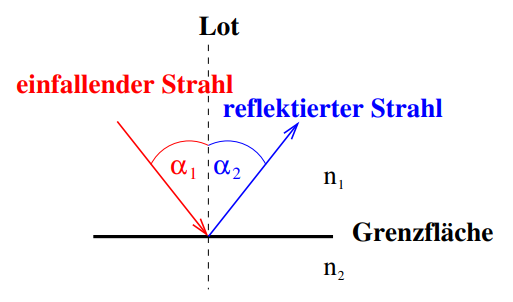
\includegraphics[width=5cm, height=3.5cm]{img/reflexion.png}
        \caption[]
        {{\small Reflexion an einer\\Grenzfläche.}}    
        \label{fig:reflexion}
    \end{subfigure}
    \hfill
    \begin{subfigure}[b]{0.3\textwidth}  
        \centering 
        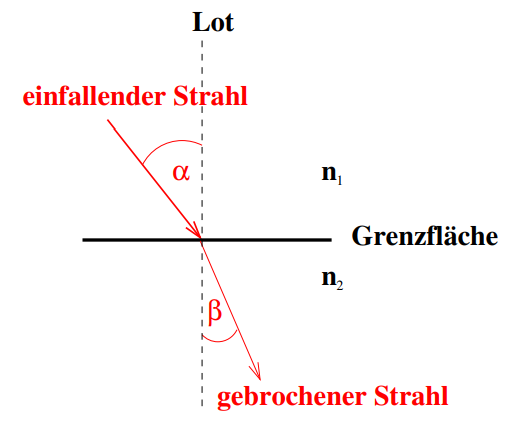
\includegraphics[width=5cm, height=4cm]{img/brechung.png}
        \caption[]
        {{\small Brechung an einer\\Grenzfläche.}}    
        \label{fig:brechung}
    \end{subfigure}
    \hfill
    \begin{subfigure}[b]{0.3\textwidth}  
        \centering 
        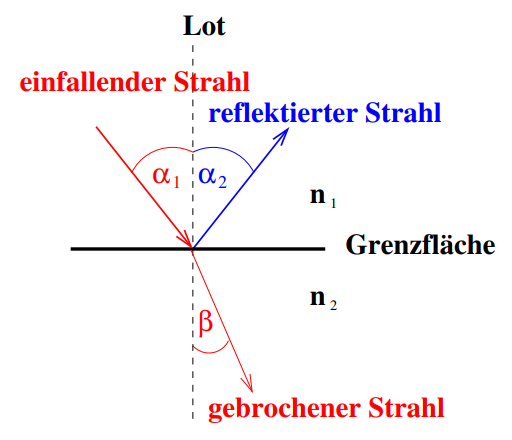
\includegraphics[width=5cm, height=4cm]{img/reflexion_transmission.png}
        \caption[]
        {{\small Reflexion und Transmission an einer Grenzfläche.}}    
        \label{fig:reflexion_transmission}
    \end{subfigure}
\end{figure}
Die Grafiken wurden der Versuchsanleitung entnommen \cite{V400}.
\subsection{Wellenoptik}
Das Phänomen der Beugung ist nicht mit der geometrischen Optik erklärbar. Um Beugung zu erklären muss die Wellennatur des Lichts beschrieben werden.
Die elektromagnetische Welle wird durch die Frequenz $f$ bzw. die Wellenlänge $\lambda$ und die Ausbreitungunsgeschwindigkeit $c$ charakterisiert.
Wellen können sich überlagern. Die Gesamtintensität der resultierenden Welle an einem Punkt ergibt sich aus der Summe der Einzelintensitäten (Superpositionsprinzip).
Wellen derselben Frequenz und einem festen Phasenbezug interferieren. Es wird unterschieden zwischen konstruktiver, einer Verstärkung, und destruktiver, einer
Abschwächung, Interferenz. Bei einem Gangunterschied von $\frac{\lambda}{2}$ und gleicher Intensität löschen sich Wellen vollständig aus.\\
Beugung kann an einer Blende oder einem Gitter beobachtet werden. Wichtig ist es, dass die Abmessungen des Gitter klein im Vergleich zur Wellenlänge sind. Das Huygen'sche 
Prinzip beschreibt die Ausbreitung:\\
\begin{itshape}
    Jeder Punkt einer Welle ist der Ausgangspunkt einer Elementarwelle gleicher Frequenz. Die Einhüllende aller Sekundärwellen stellt zu einem späteren Zeitpunkt die
    neue Lage der Wellenfront dar.
\end{itshape}
Das naheliegenste ist es die Beugung am Einzelspalt herbeizuführen. Trifft monochromatisches Licht auf den Spalt der breite $a$, so wird das Licht nach dem Huygen'schen 
Prinzip gebeugt. Die neuen Wellenfronten haben folglich dieselbe Frequenz und einen festen Phasenbezug. In einem Abstand $L$ befindet sich ein Schirm, auf dem ein 
Interferenzmuster zu beobachten ist. Die Intensitätsmaxima befinden sich an den Stellen, für die gilt:
\begin{equation*}
    a \cdot sin(\alpha) = k\cdot\lambda.
\end{equation*}
Das $k$ ist dabei eine natürliche Zahl und gibt das $k\text{-te}$ Intensitätsmaxima an. In \autoref{einzelspalt} ist eine solche Messung simuliert.
\begin{figure}[H]
    \centering
    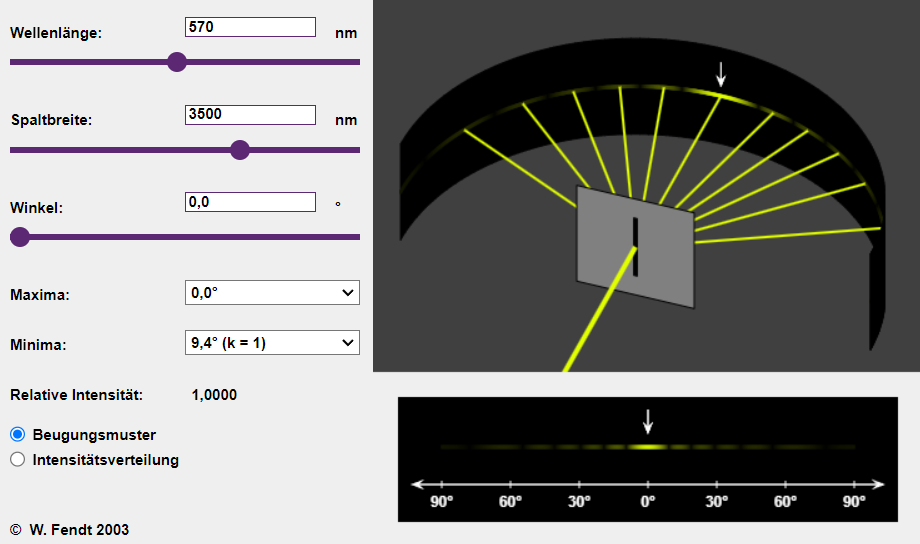
\includegraphics[width=\textwidth]{img/beugung.png}
    \caption{Beugung am Einfachspalt \cite{Einzelspalt}.}
    \label{einzelspalt}
\end{figure}
Analog lässt sich ein Gesetz für ein Gitter mit N-Einzelspalten mit Gitterkonstante $d$ formulieren:
\begin{equation*}
    d \cdot sin(\alpha) = k\cdot\lambda.
\end{equation*}
